\documentclass{beamer}

\mode<presentation>
{
  \usetheme{CambridgeUS}      % or try Darmstadt, Madrid, ...
  \usecolortheme{default} % or try albatross, beaver, crane, ...
  \usefonttheme{default}  % or try serif, structurebold, ...
  \setbeamertemplate{navigation symbols}{}
  \setbeamertemplate{caption}[numbered]
} 

\usepackage[english]{babel}
\usepackage[utf8x]{inputenc}
\usepackage{listings}
\usepackage[ampersand]{easylist}



\definecolor{KTI_green}{RGB}{150, 189, 13}
\definecolor{TU_red}{RGB}{255, 55, 81}
\definecolor{faint_gray}{RGB}{180, 180, 180}

\definecolor{syntax_green}{rgb}{0,0.6,0}
\definecolor{syntax_gray}{rgb}{0.9, 0.9, 0.9}
\definecolor{syntax_mauve}{rgb}{0.58,0,0.82}

\lstset{ 
  backgroundcolor=\color{syntax_gray},  % choose the background color
  basicstyle=\scriptsize\ttfamily,        		% size of fonts used for the code
  breaklines=false,                		% automatic line breaking only at whitespace
  captionpos=b,                    		% sets the caption-position to bottom
  commentstyle=\color{syntax_green},    % comment style
  escapeinside={\%*}{*)},          		% if you want to add LaTeX within your code
  keywordstyle=\color{blue},       		% keyword style
  stringstyle=\color{syntax_mauve},     % string literal style
  columns=fullflexible,
  frame=single,
  framesep=0.5cm,
  framexleftmargin=0.5cm,
  xleftmargin=0.5cm,
  framexrightmargin=0.5cm,
  xrightmargin=0.5cm,
  frame=tb,                 
    numbers=left,                    
    numbersep=15pt,  
  }
  
  
\newcommand{\logopython}{\raggedleft 
\includegraphics[height=0.5cm]{logo_python}\hspace{0.1cm}\\\raggedright}
\newcommand{\logopythonbottom}{\raggedleft\vspace{-0.8cm}
\includegraphics[height=0.5cm]{logo_python}\hspace*{0.05cm}\\\raggedright}

\title[BSP18 - Restgeld]{Restgeld}
\author{Dickbauer Y., Moser P., Perner M.}
\institute{PS Computergestützte Modellierung, WS 2016/17}
%\date{Date of Presentation}

\begin{document}

\begin{frame}
  \titlepage
\end{frame}

\begin{frame}{Outline}
  \tableofcontents
\end{frame}

\section{Aufgabenstellung}
\begin{frame}{Aufgabenstellung}
30 Besucher wollen zu einer Veranstaltung. Der Eintritt zur Veranstaltung beträgt 5
Euro. Die Besucher der Veranstaltung können entweder mit 5-Euro oder 10-Euro-Scheinen
bezahlen. In der Kasse liegt zu Beginn eine konfigurierbare Anzahl an 5-Euro-Scheinen.

\begin{block}{Grundproblem}
Die Wahrscheinlichkeit, dass ein Besucher mit einem 10-Euro-Schein bezahlen
möchte, beträgt 60 Prozent, dass ein Besucher mit einem 5-Euro-Schein bezahlen
möchte, beträgt 40 Prozent.   
\end{block}

\begin{block}{Alternative}
Es gibt 15 Personen mit einem 10 Euro-Schein und 15 Personen mit einem
5 Euro-Schein, die in zufälliger Reihenfolge zur Kasse kommen.
\end{block}
\end{frame}


\begin{frame}{Aufgabenstellung}
Stellen Sie bei den einzelnen Alternativen mittels Simulation fest, ob jeweils genug 5-
Euro-Scheine in der Kasse sind, damit die Besucher mit 10-Euro-Schein das Restgeld
bekommen. Stellen Sie fest, ob bzw. wie viele Besucher warten müssen und wie lange sie
warten müssen bzw. ob Besucher am Ende sogar ohne Restgeld übrig bleiben. Stellen Sie
im Rahmen der Präsentation den Ablauf des Programmes anhand von selbstgewählten
Zufallszahlen vor.

\begin{itemize}
  \item Eingabe: Anzahl an 5-Euro-Scheinen zu Beginn
  \item Output: Je Runde Geldschein, mit dem der Kunde bezahlen möchte, und Anzahl
an 5- und 10-Euro-Scheinen in der Kasse.
\end{itemize}
\end{frame}


\section{Flow Chart}
\begin{frame}{Flow Chart Hauptprogramm Grundproblem}
	\centering
  	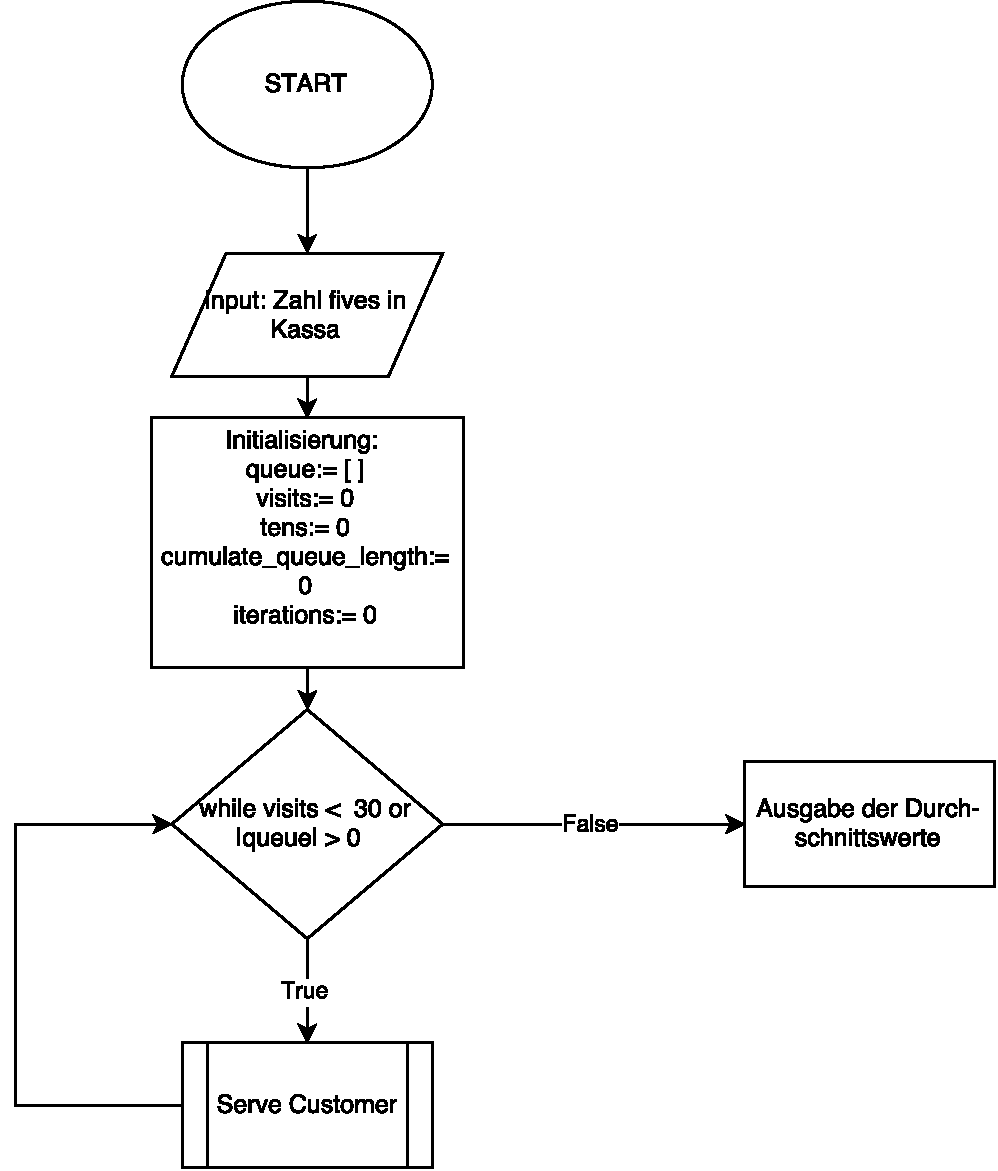
\includegraphics[scale=0.4]{BSP18_Flow_Chart_1.pdf}
\end{frame}

\begin{frame}{Flow Chart Unterprozess Serve Customer}
	\centering
  	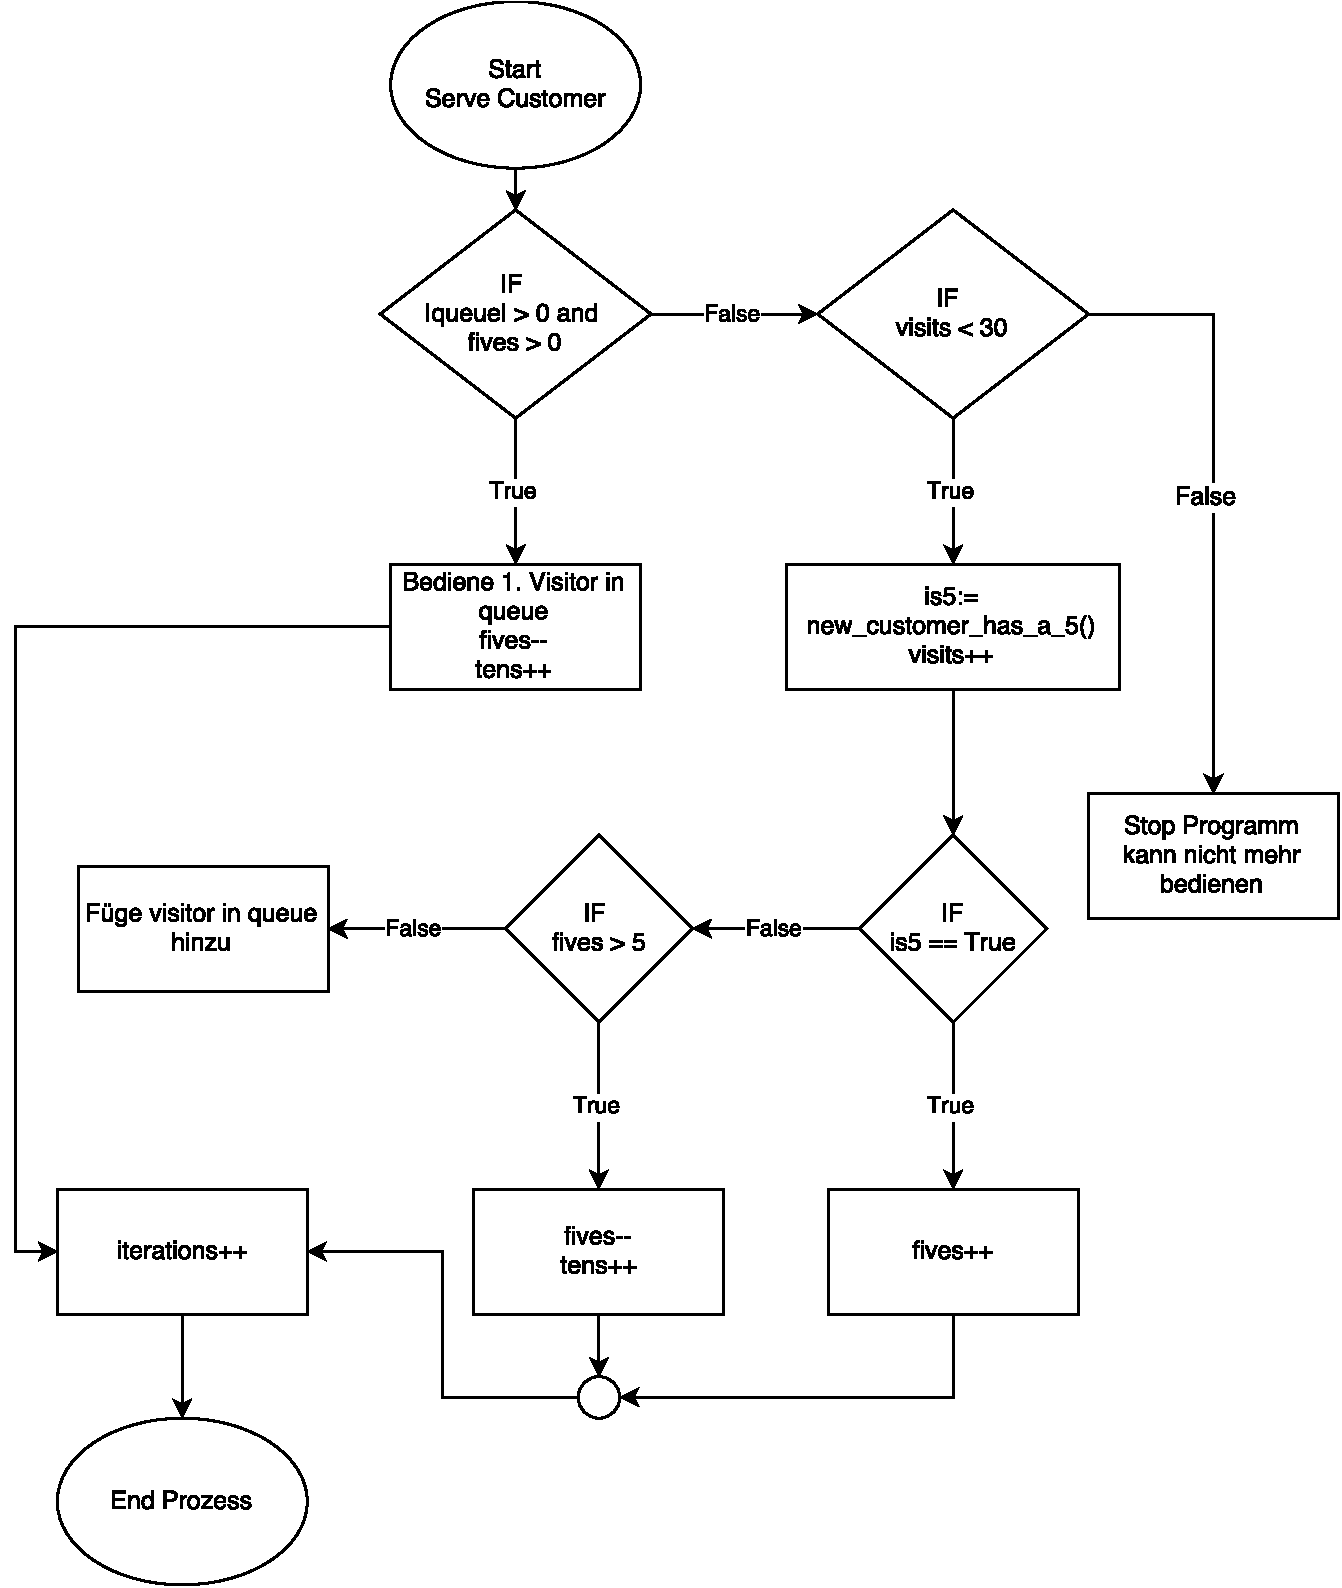
\includegraphics[scale=0.25]{BSP18_Flow_Chart_2.pdf}
\end{frame}

\begin{frame}{Flow Chart Unterprozess new\_customer\_has\_a\_5() inklusive Alternative}
	\centering
  	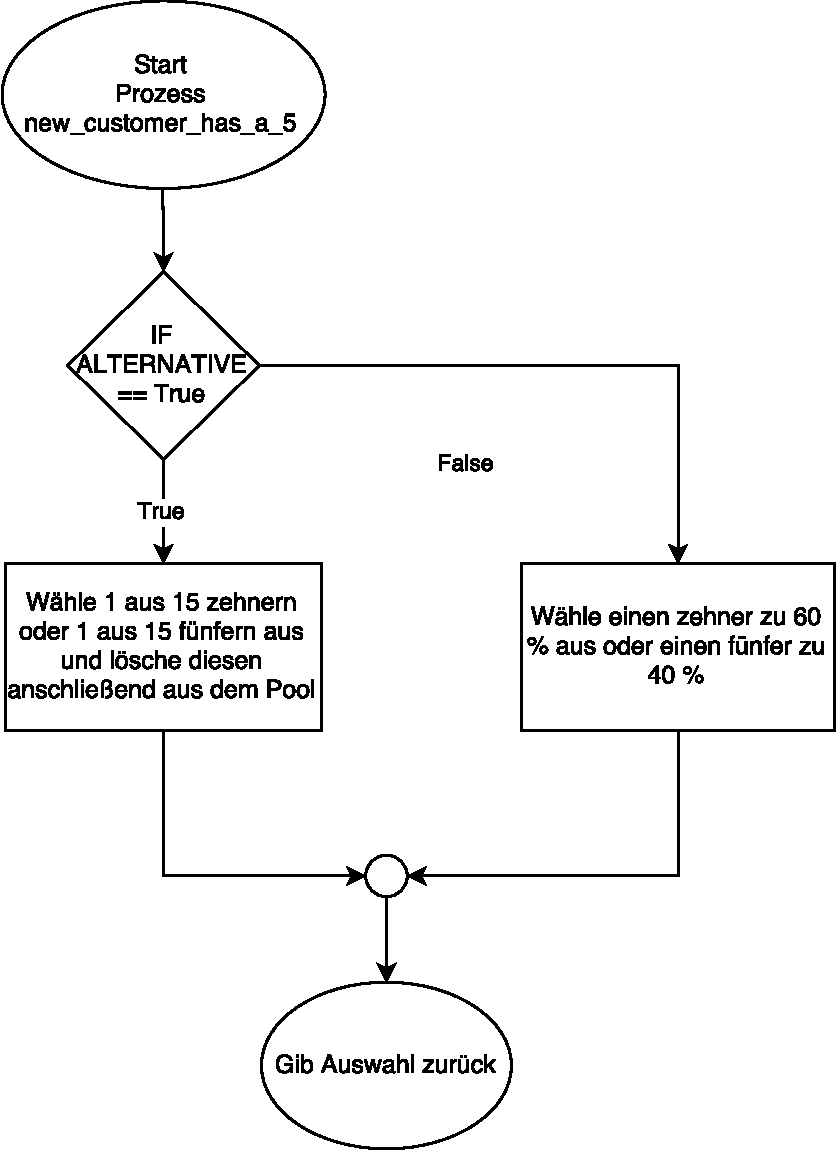
\includegraphics[scale=0.3]{BSP18_Flow_Chart_3.pdf}
\end{frame}


\subsection{Verwendete Funktionen}
% \begin{frame}[fragile]{Funktion euclidean\_distance(p1, p2)}
  \begin{itemize}
    \item Diese Funktion verlangt zwei Punkte (x1, y1) (x2, y2) als Eingabeparameter
    \item Gibt die eukliedsche Distanz zurück
  \end{itemize}
  \begin{lstlisting}[language=python]
def euclidean_distance(point_1, point_2):
    """
        Calculates the euclidean distance between two points
        
        point_1: a tuple of (x,y) values
        point_2: a tuple of (x,y) values
    """
    delta_x = point_2[0] - point_1[0]
    delta_y = point_2[1] - point_1[1]
    return (delta_x ** 2 + delta_y ** 2) ** 0.5
\end{lstlisting}
\logopythonbottom
\end{frame}	
%\begin{frame}[fragile]{Funktion random\_number\_from\_interval(..)}
  \begin{itemize}
    \item Diese Funktion verlangt zwei Eingabeparameter \textit{lower} und \textit{upper}
    \item Gibt eine (pseudo)Zufallszahl (\textit{float}) im Intervall  [\textit{lower}, \textit{upper}) zurück 
    \item \textit{random.random()} ist eine Funktion der Python Standardbibliothek, welche ein Zufallszahl (\textit{float}) im Intervall [\textit{lower}, \textit{upper}) zurück gibt
    \item Mersenne Twister Methode wird als Generator der ZZ verwendet\footnote[frame] {\scriptsize\url{https://docs.python.org/3.5/library/random.html}} \footnote[frame] {\scriptsize\url{https://en.wikipedia.org/wiki/Mersenne_Twister}}
  \end{itemize}
  \begin{lstlisting}[language=python]
def random_number_from_interval(lower, upper):
    val = random.random()
    return lower + (upper -lower) * val
\end{lstlisting}
\logopythonbottom
\end{frame}	

 \begin{frame}[fragile]{Funktion random\_std(..)}
  \begin{itemize}
    \item Diese Funktion verlangt zwei optionale Parameter: $\mu$ und $\sigma$ welche per default auf 0 und 1 gesetzt sind
    \item Gibt eine normalverteilte Zufallszahl zurück
    \item Analog zur Folie im Unterricht
  \end{itemize}
  \begin{lstlisting}[language=python]
def random_std(mean=0, sigma=1):
    """Returns a normally distrubed random number"""
    u1, u2 = random.random(), random.random()
    zz = (-2 * log(u1))**(1/2) * sin(2 * pi * u2)
    return sigma * zz + mean
\end{lstlisting}
\logopythonbottom
\end{frame}	


\end{document}
